%%%%%%%%%%%%%%%%%%%
% SECTION: 3DCNN
%%%%%%%%%%%%%%%%%%%
\section{3D Convolutional Neural Networks}

A conventional CNN uses spatial information learned from an image but cannot learn temporal information. A 3D CNN, on the contrary, extracts features from both spatial and temporal dimensions ; thus a 3D CNN can be used with videos by using the extra temporal dimension. This is obtained by accomplishing 3D convolutions that also captures the information of a series of frames. The 3D CNN encapsulates information from the temporal channels (frames) and the spatial channels (RGB) and combines them in a feature representation. \cite{Ji3DRecognition}

% FIGURE: 3D CNN
\begin{figure}[!htb]	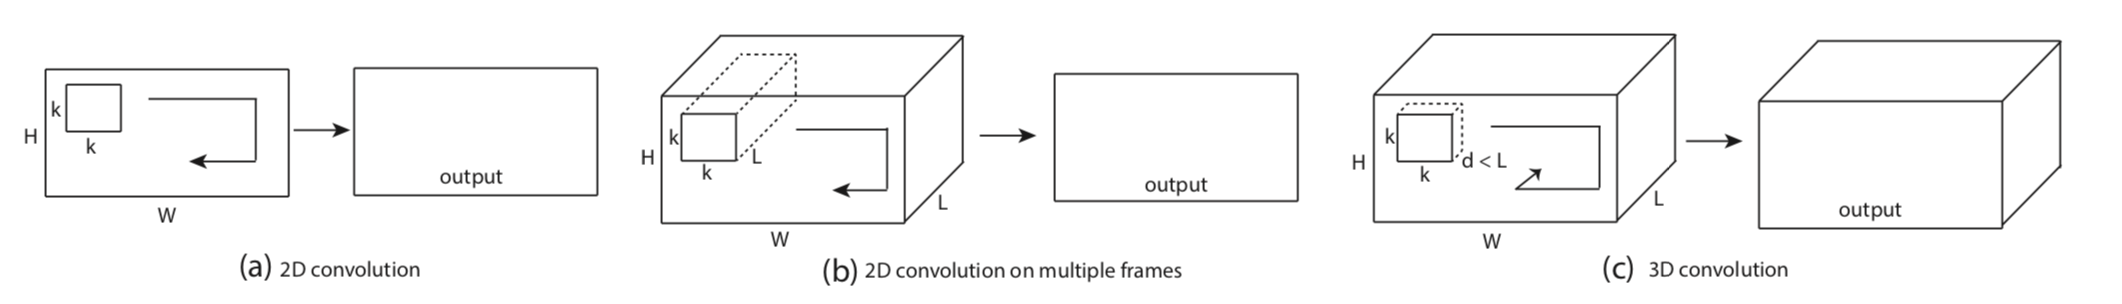
\includegraphics[width=0.9\textwidth]{images/3dcnn.png} 
    \centering

\caption{
Differences between a 2D CNN, 2D CNN with multiple frames and a 3D CNN. \cite{Tran2015LearningNetworks}
} 

\label{fig:3dcnn}
\end{figure}

The 3D convolution is obtained from a 3D kernel that convolves multiple contiguous frames that are stacked together. The features extracted are connected to the contiguous frames in the previous layer and is this exact process that captures the temporal information. The equation \ref{eq:3dcnn} gives the value in a given position $(x,y,z)$ in the $j$th feature map and in the $i$th layer; $R{_i}$ is the size of the kernel and $w_{ijm}^{pqr}$ is the $(pqr)$th value connected to the $m$th feature map of the previous layer. \cite{Tran2015LearningNetworks}

\begin{equation} \label{eq:3dcnn}
v^{_{ij}^{xyz}} = tanh\left ( b_{ij} + \sum_{m}\sum_{p=0}^{P_{i}-1}\sum_{q=0}^{Q_{i}-1}\sum_{r=0}^{R_{i}-1}  w_{ijm}^{pqr} v_{(i-1)m}^{(x+p)(y+q)(z+r)} \right )
\end{equation}

Like a 2D CNN, only one type of features can be extracted from a stack of frames. This is because the kernel weights are replicated across the video. To obtain multiple types of features, various convolutions with different kernels can be applied to the same spot in the previous layer. This generates a large number of feature maps with different types of features.

% FIGURE: 3D Convolution
\begin{figure}[!htb]	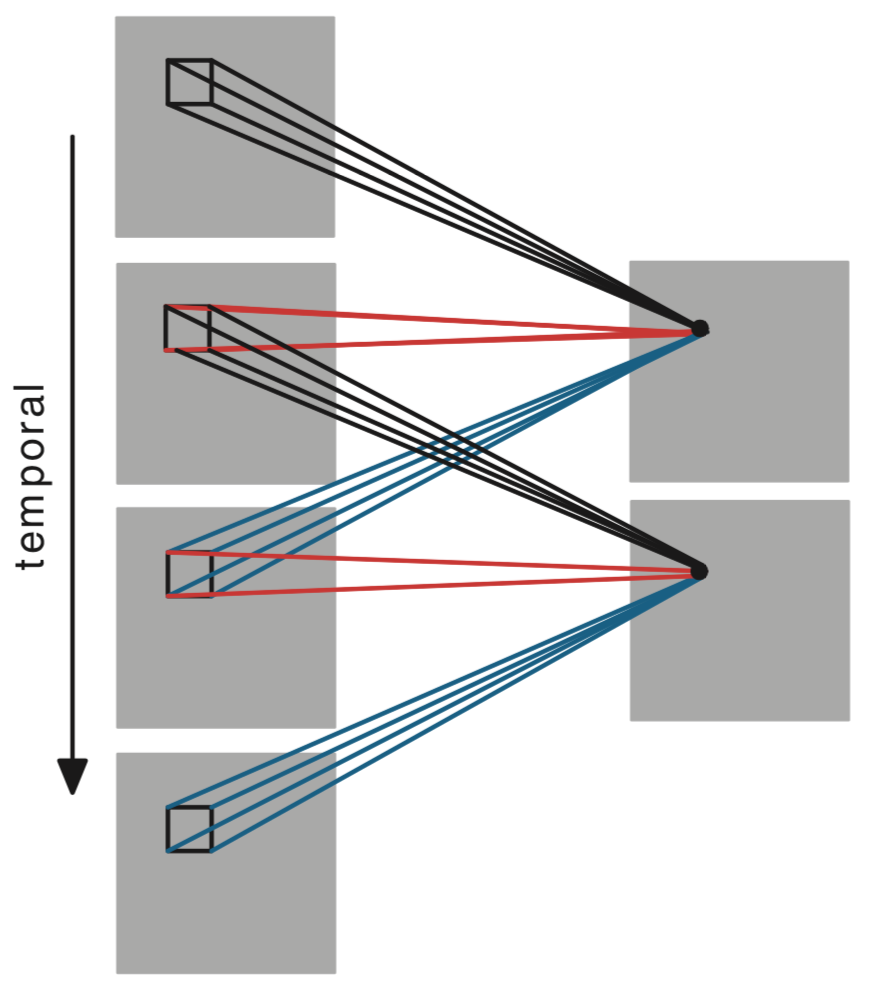
\includegraphics[width=0.4\textwidth]{images/3d_convolution.png} 
    \centering

\caption{
The 3D kernel is applied in the input video to extract temporal features. \cite{Tran2015LearningNetworks}
} 

\label{fig:3d_convolution}
\end{figure}